\documentclass[conference]{IEEEtran}
\IEEEoverridecommandlockouts
% The preceding line is only needed to identify funding in the first footnote. If that is unneeded, please comment it out.
%Template version as of 6/27/2024

\usepackage{cite}
\usepackage{amsmath,amssymb,amsfonts}
\usepackage{algorithmic}
\usepackage{graphicx}
\usepackage{textcomp}
\usepackage{xcolor}
\def\BibTeX{{\rm B\kern-.05em{\sc i\kern-.025em b}\kern-.08em
    T\kern-.1667em\lower.7ex\hbox{E}\kern-.125emX}}
\renewcommand{\abstractname}{Resumen}

\begin{document}

\title{Sistema de relevamiento digital para fiscalización pesquera mediante procesamiento digital de imágenes}

\author{\IEEEauthorblockN{Santiago Bargas}
\IEEEauthorblockA{santidariobargas@hotmail.com}
\and\IEEEauthorblockN{Segundo Saccanni}
\IEEEauthorblockA{segundosaccanni@gmail.com}
}

\maketitle

\begin{abstract}
Este trabajo presenta un sistema de relevamiento digital orientado a la fiscalización pesquera en puntos de desembarco del río Paraná, que procesa fotografías de individuos sobre una superficie plana para segmentarlos, rectificar su orientación y clasificar la especie a la que pertenecen. El sistema se desarrolla y valida sobre el dataset público AutoFish, utilizando técnicas clásicas de visión por computadora (umbralización de Otsu, morfología, transformación de perspectiva) para las etapas de preprocesamiento y rectificación, y un modelo YOLOv8n-cls para la clasificación de especies. Se obtuvo una precisión top-1 cercana al 97\% sobre el conjunto de validación, evaluada además sobre un conjunto de test completamente ciego. Se discuten las limitaciones encontradas —principalmente errores de orientación y confusión entre individuos y fondo— y las mejoras propuestas para la captura de datos propios en el río Paraná.
\end{abstract}

\section{Introducción}

\subsection{Contexto y motivación}
En los puntos de desembarco pesquero del río Paraná, los organismos de fiscalización deben relevar de forma manual la especie y el tamaño de los individuos capturados, con el objetivo de controlar el cumplimiento de tallas mínimas y cupos por especie. Este relevamiento manual es lento, depende de la experiencia del fiscalizador y resulta difícil de estandarizar entre distintos puntos de control. Una alternativa es contar con un sistema que, a partir de una fotografía tomada con un dispositivo móvil, permita identificar automáticamente cada individuo presente en la imagen, reconocer su especie y estimar sus dimensiones, agilizando el proceso y reduciendo la subjetividad del relevamiento.

\subsection{Objetivos}
El objetivo general de este trabajo es desarrollar un sistema de procesamiento digital de imágenes capaz de, a partir de una fotografía de individuos pesqueros sobre una superficie plana, (i) separar el fondo y aislar cada individuo presente en la imagen, (ii) llevar cada individuo a una orientación canónica común, (iii) clasificar la especie de cada individuo y (iv) estimar sus medidas morfológicas a partir de un objeto de referencia. En este trabajo se priorizó el desarrollo y validación de las tres primeras etapas, dejando la estimación de talla en unidades físicas y la generación de la salida final como trabajo en curso, a la espera de un dataset propio con objeto de referencia.

\subsection{Trabajos relacionados}
Para el desarrollo y la validación del sistema se utilizó el dataset público AutoFish \cite{b1}, generado a partir de imágenes de una cinta transportadora de un punto de desembarco pesquero, que provee máscaras de segmentación de instancia, cajas delimitadoras, especie y largo real de cada individuo. La etapa de clasificación de especies se implementó utilizando la arquitectura YOLOv8 en su variante de clasificación \cite{b2}, mientras que las etapas de segmentación y rectificación se basan en técnicas clásicas de procesamiento de imágenes, como la umbralización de Otsu \cite{b3} y operaciones morfológicas y geométricas implementadas con OpenCV \cite{b4}.

\section{Materiales y métodos}

\subsection{Dataset}
Se utilizó el dataset AutoFish \cite{b1}, compuesto por aproximadamente 1500 imágenes de una cinta transportadora con un total de 18160 máscaras de segmentación de instancia correspondientes a 454 individuos distintos, distribuidos en 7 especies (\emph{cod}, \emph{haddock}, \emph{whiting}, \emph{hake}, \emph{horse mackerel}, \emph{saithe} y \emph{other}). El dataset está organizado en 25 grupos (\texttt{group\_01} a \texttt{group\_25}), cada uno con dos subconjuntos sin solapamiento (\texttt{Set1} y \texttt{Set2}) y un subconjunto con solapamiento intencional (\texttt{All}). Para este trabajo se utilizaron únicamente las imágenes sin solapamiento, ya que el pipeline propuesto asume individuos aislados. Para cada individuo, el archivo de anotaciones provee su máscara de segmentación, su caja delimitadora, su especie, su largo real en centímetros y el lado del cuerpo visible en la imagen (\texttt{side\_up}), información utilizada tanto para construir el dataset de entrenamiento como para evaluar el sistema.

\subsection{Pipeline propuesto}
El sistema se organiza en seis etapas secuenciales: (1) entrada de la imagen y sus anotaciones, (2) preprocesamiento para separar el fondo y detectar cada individuo, (3) rectificación de la orientación de cada individuo, (4) clasificación de la especie mediante un modelo entrenado, (5) estimación de las medidas morfológicas de cada individuo y (6) generación de una salida estructurada con la especie y las medidas correspondientes a cada individuo de la imagen. En este trabajo se implementaron y validaron las etapas 1 a 4 sobre el dataset AutoFish, mientras que las etapas 5 y 6 se encuentran implementadas a nivel de medidas en píxeles, pendientes de calibración con un objeto de referencia físico.

\subsection{Etapa 1: Imagen de entrada}
Esta etapa carga la imagen original junto con la información de anotaciones asociada a cada individuo presente en ella: identificador, caja delimitadora, máscara de segmentación, especie, largo real y lado del cuerpo visible. Esta información se utiliza como referencia (\emph{ground truth}) durante el desarrollo y la evaluación, pero no es requerida por el pipeline final, que opera únicamente sobre la imagen capturada.

\subsection{Etapa 2: Preprocesamiento}
La etapa de preprocesamiento separa el fondo de la cinta transportadora de los individuos presentes en la imagen y obtiene, para cada uno, un rectángulo rotado que delimita su posición. El procedimiento consta de los siguientes pasos: (i) conversión de la imagen a escala de grises, (ii) suavizado mediante un filtro gaussiano de $7\times7$ para reducir el ruido de la textura del fondo, (iii) umbralización binaria mediante el método de Otsu \cite{b3}, que determina automáticamente el umbral que separa los individuos (más oscuros) del fondo (más claro), (iv) limpieza morfológica mediante una operación de apertura seguida de una de cierre, con un elemento estructurante en forma de cruz de $35\times35$ píxeles, para eliminar ruido residual y cerrar pequeños huecos, (v) detección de los contornos externos de la máscara resultante y (vi) filtrado de los contornos cuya área sea menor a 25000 píxeles, descartando artefactos pequeños. Para cada contorno válido se ajusta un rectángulo rotado mínimo, que define la posición, el tamaño y la orientación de cada individuo detectado.

\subsection{Etapa 3: Rectificación}
A partir del rectángulo rotado obtenido en la etapa anterior, se aplica una transformación de perspectiva para recortar y enderezar cada individuo de forma que quede orientado horizontalmente. Sobre el recorte resultante se estima en qué extremo se encuentra la cabeza, comparando el grosor de la máscara entre el primer y el último tercio del recorte —el extremo más grueso corresponde a la cabeza (ojo y opérculo)— y se aplica, de ser necesario, un espejado horizontal para que la cabeza quede siempre del lado izquierdo. Luego se estima la orientación vertical del hocico, comparando la posición del punto más extremo de la cabeza respecto del centro vertical de dicha región, y se aplica un espejado vertical para que el hocico quede siempre orientado hacia abajo. De esta manera, todos los individuos quedan llevados a una orientación canónica común (cabeza a la izquierda, hocico hacia abajo), independientemente de su posición y orientación original en la imagen. Estos criterios se calculan únicamente a partir de la máscara de cada individuo, por lo que son aplicables al pipeline final sobre fotografías de campo, sin depender de información de anotaciones.

\subsection{Etapa 4: Clasificación}
La clasificación de especies se realiza mediante un modelo YOLOv8n-cls \cite{b2}, una variante liviana de clasificación de la familia YOLOv8. Para entrenarlo se generó un dataset de recortes individuales aplicando las etapas 1 a 3 sobre todas las imágenes sin solapamiento del dataset, obteniendo 8016 recortes organizados por especie. El conjunto se dividió en tres particiones por grupo de imágenes: entrenamiento (\texttt{group\_01} a \texttt{group\_16}, 64\%, 5286 imágenes), validación (\texttt{group\_17} a \texttt{group\_20}, 16\%, 1184 imágenes), utilizada para el monitoreo y el criterio de parada temprana, y test (\texttt{group\_21} a \texttt{group\_25}, 20\%, 1546 imágenes), utilizado únicamente para la evaluación final y no visto durante el entrenamiento.

Durante el entrenamiento se aplicaron técnicas de aumentación de datos seleccionadas en función de las características del problema: variaciones de brillo (\texttt{hsv\_v}=0.4) para representar distintas condiciones de iluminación durante el desembarco, variaciones de tono y saturación (\texttt{hsv\_h}=0.015, \texttt{hsv\_s}=0.7) para representar la variabilidad natural de coloración entre individuos de una misma especie, recorte parcial aleatorio (\texttt{erasing}=0.4) para simular individuos parcialmente fuera de cuadro u ocluidos por otros, y espejado vertical (\texttt{flipud}=0.5) para que el modelo sea robusto frente a los errores de orientación de la etapa 3, que dejan aproximadamente uno de cada diez individuos con el hocico hacia arriba. El espejado horizontal (\texttt{fliplr}) se desactivó deliberadamente, ya que la etapa de rectificación garantiza que todos los individuos lleguen con la cabeza hacia la izquierda, y entrenar con individuos con la cabeza hacia la derecha introduciría una variabilidad que nunca se presenta en producción.

El modelo se entrenó durante un máximo de 50 épocas, con un criterio de parada temprana de 10 épocas sin mejora en el conjunto de validación (\texttt{patience}=10), tamaño de lote de 64, tamaño de imagen de entrada de $224\times224$ píxeles y semilla fija para garantizar la reproducibilidad.

\subsection{Etapa 5: Estimación de talla}
A partir del recorte rectificado de cada individuo, sus dimensiones en píxeles (largo y ancho) se obtienen directamente del tamaño del rectángulo ajustado en la etapa de preprocesamiento. Para convertir estas medidas a unidades físicas (centímetros) es necesario contar con un objeto de referencia de tamaño conocido en la misma fotografía, condición prevista para la captura de datos pero no disponible en el dataset AutoFish utilizado en este trabajo. Esta calibración queda planteada como trabajo futuro, a realizar sobre el dataset propio a capturar en el río Paraná.

\subsection{Etapa 6: Salida}
La etapa final integra los resultados de las etapas anteriores y genera, para cada individuo detectado en la imagen, un registro con su especie predicha, la confianza de la predicción y sus medidas en píxeles (largo y ancho), exportado en formato estructurado. Esta salida constituye la base sobre la que, una vez disponible la calibración de escala, se incorporarán las medidas en unidades físicas y la correlación peso/edad.

\section{Resultados}

\subsection{Preprocesamiento y rectificación}
La Fig. \ref{fig:pipeline} muestra el resultado de aplicar las etapas 1 a 3 sobre una imagen de ejemplo: la imagen original con múltiples individuos, la máscara binaria obtenida tras la umbralización y la limpieza morfológica, los individuos detectados mediante sus rectángulos rotados, y ejemplos de recortes ya rectificados con orientación canónica (cabeza a la izquierda, hocico hacia abajo).

\begin{figure}[h]
    \centering
    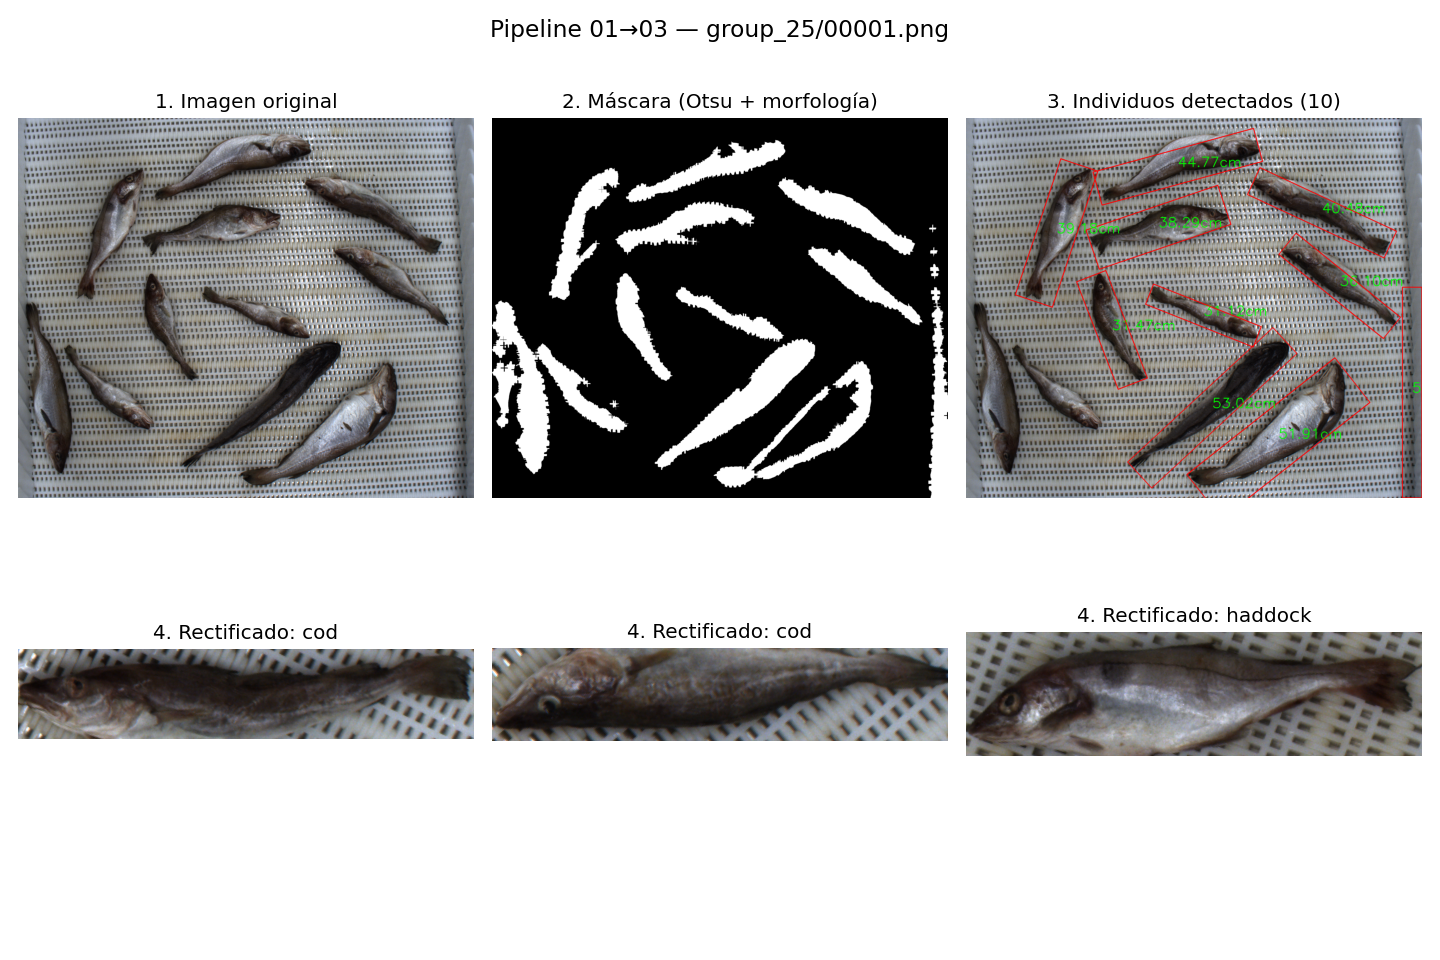
\includegraphics[width=\linewidth]{../resultados/figuras/pipeline.png}
    \caption{Etapas de preprocesamiento y rectificación: imagen original, máscara obtenida, individuos detectados y ejemplos de recortes rectificados.}
    \label{fig:pipeline}
\end{figure}

\subsection{Entrenamiento del clasificador}
La Fig. \ref{fig:curvas} muestra la evolución de la función de pérdida sobre los conjuntos de entrenamiento y validación, junto con la precisión top-1 sobre el conjunto de validación a lo largo de las épocas. El modelo alcanzó una precisión top-1 de 74.7\% en la primera época, superando el 97\% a partir de la décima época, con un máximo de 97.4\% en la época 25. El entrenamiento finalizó por criterio de parada temprana en la época 35, con una precisión top-1 de 97.1\% y una precisión top-5 cercana al 99.9\% de forma sostenida.

\begin{figure}[h]
    \centering
    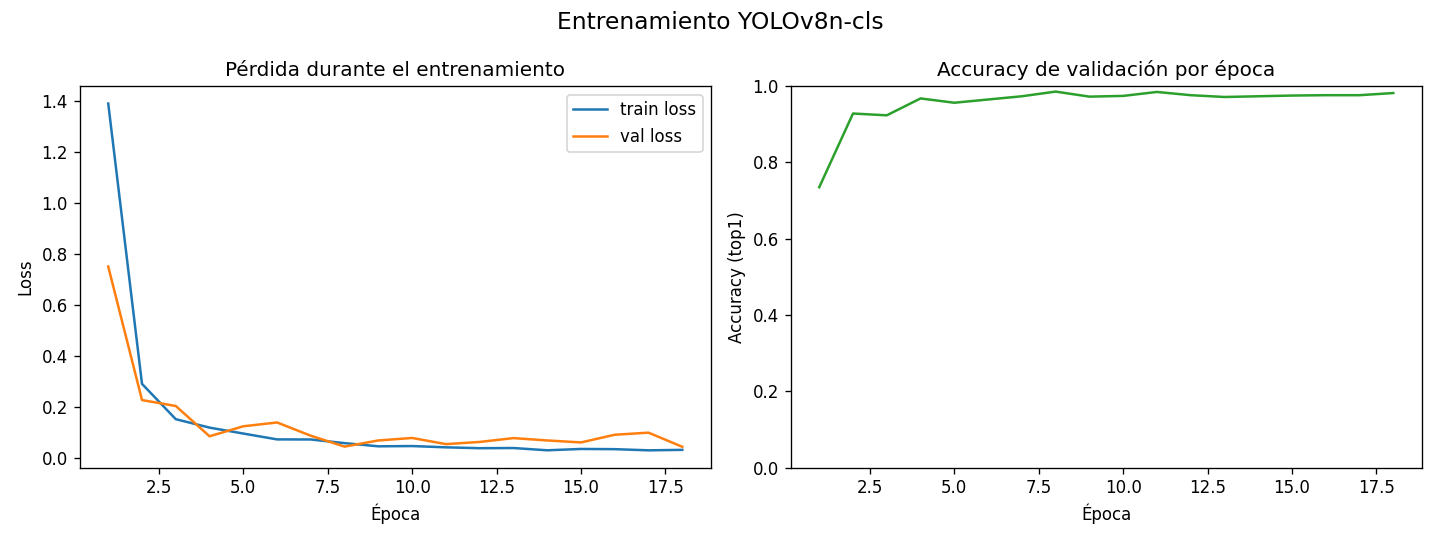
\includegraphics[width=\linewidth]{../resultados/figuras/curvas_entrenamiento.png}
    \caption{Evolución de la función de pérdida y de la precisión top-1 sobre el conjunto de validación durante el entrenamiento.}
    \label{fig:curvas}
\end{figure}

\subsection{Evaluación sobre el conjunto de test ciego}
El modelo entrenado se evaluó sobre el conjunto de test ciego (\texttt{group\_21} a \texttt{group\_25}, 1546 imágenes), no utilizado en ninguna etapa del entrenamiento. La Fig. \ref{fig:confusion} muestra la matriz de confusión normalizada por clase real, donde la diagonal representa la proporción de individuos correctamente clasificados para cada especie. La Fig. \ref{fig:predicciones} presenta ejemplos individuales de clasificación, indicando la especie real, la especie predicha y la confianza del modelo para cada caso.

\begin{figure}[h]
    \centering
    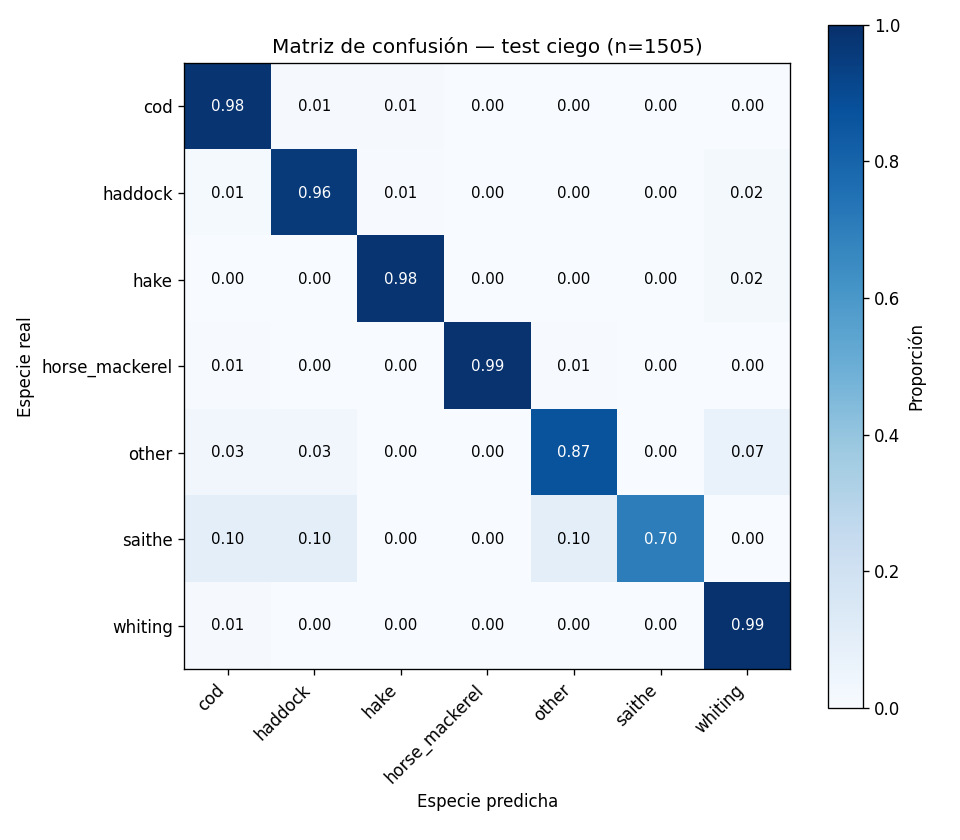
\includegraphics[width=\linewidth]{../resultados/clasificacion_yolov8n/evaluaciones/test1/matriz_confusion.png}
    \caption{Matriz de confusión normalizada sobre el conjunto de test ciego (group\_21 a group\_25).}
    \label{fig:confusion}
\end{figure}

\begin{figure}[h]
    \centering
    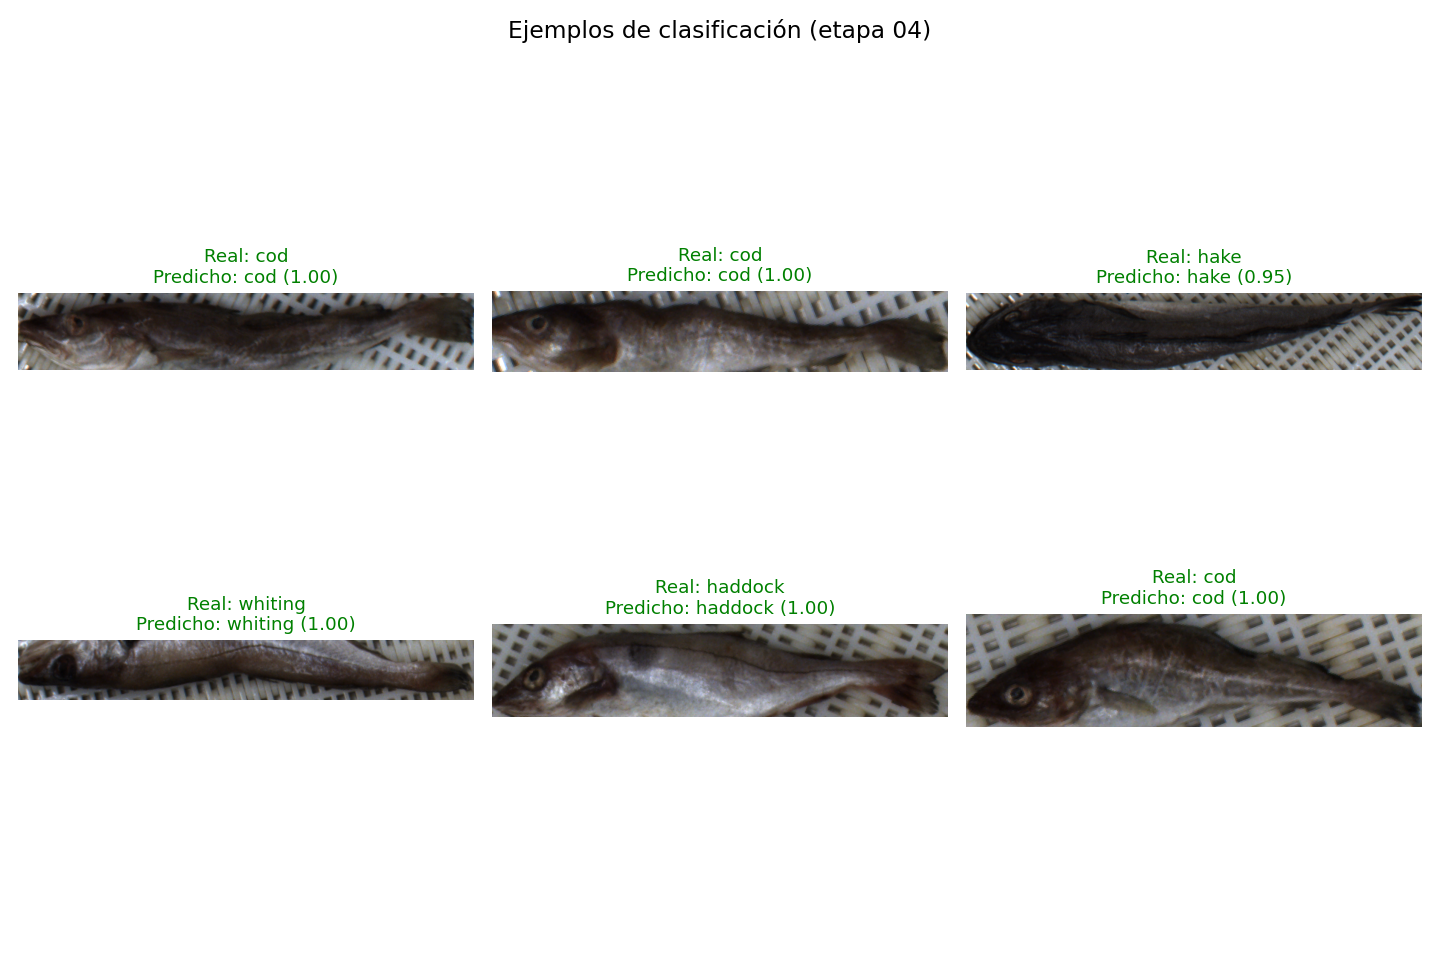
\includegraphics[width=\linewidth]{../resultados/clasificacion_yolov8n/evaluaciones/test1/predicciones.png}
    \caption{Ejemplos de clasificación sobre individuos rectificados, indicando especie real, especie predicha y confianza.}
    \label{fig:predicciones}
\end{figure}

\section{Discusión}
Durante el desarrollo se identificaron dos limitaciones principales. La primera es la confusión entre individuo y fondo en la etapa de preprocesamiento cuando el individuo presenta una zona ventral muy clara o plateada, de tonalidad similar al fondo de la cinta transportadora, lo que puede afectar la segmentación basada en umbralización. La segunda es un error de orientación en la etapa de rectificación: aproximadamente uno de cada diez individuos queda con el hocico hacia arriba en lugar de hacia abajo, debido a casos límite en la estimación del extremo de la cabeza a partir de la máscara. Este segundo problema se mitigó parcialmente mediante la aumentación con espejado vertical durante el entrenamiento del clasificador, de modo que el modelo es robusto ante individuos en ambas orientaciones verticales.

Ambas limitaciones están vinculadas a las condiciones de captura de la imagen. Un fondo de color uniforme y de alto contraste con respecto a los individuos —por ejemplo, una superficie de color verde, poco habitual en las especies del río Paraná— simplificaría la segmentación y reduciría la confusión entre individuo y fondo, mejorando además indirectamente la precisión de la etapa de rectificación.

\section{Conclusiones}
Se desarrolló un pipeline de procesamiento digital de imágenes capaz de separar el fondo, aislar y rectificar la orientación de individuos pesqueros, y clasificar su especie con una precisión cercana al 97\% sobre un conjunto de test ciego, utilizando técnicas clásicas de visión por computadora combinadas con un modelo de clasificación liviano (YOLOv8n-cls). Los resultados obtenidos sobre el dataset AutoFish validan el enfoque propuesto para las etapas de segmentación, rectificación y clasificación, mientras que la estimación de talla en unidades físicas y la generación de la salida final quedan condicionadas a la disponibilidad de un objeto de referencia en la imagen.

\section{Trabajo futuro}
Como continuación de este trabajo se prevé incorporar un dataset propio capturado en puntos de desembarco del río Paraná, que incluya un objeto de referencia de tamaño conocido en cada fotografía para calibrar la conversión de medidas en píxeles a unidades físicas, y un fondo de color contrastante que facilite la segmentación. Asimismo, se planea medir de forma sistemática la tasa de error de orientación de la etapa de rectificación comparando con la información de referencia disponible, y abordar el caso de individuos solapados mediante técnicas de segmentación de instancias. Finalmente, una vez disponibles las medidas en unidades físicas, se buscará incorporar un modelo de correlación entre talla, peso y edad de cada individuo.

\begin{thebibliography}{00}
\bibitem{b1} M. M. Bengtson \emph{et al.}, ``AutoFish: Dataset and Benchmark for Fine-grained Analysis of Fish,'' arXiv:2501.03767, 2025.

\bibitem{b2} G. Jocher, A. Chaurasia, J. Qiu, ``Ultralytics YOLOv8,'' 2023. [Online]. Disponible: https://github.com/ultralytics/ultralytics

\bibitem{b3} N. Otsu, ``A threshold selection method from gray-level histograms,'' IEEE Trans. Syst. Man Cybern., vol. 9, no. 1, pp. 62--66, 1979.

\bibitem{b4} G. Bradski, ``The OpenCV Library,'' Dr. Dobb's Journal of Software Tools, 2000.

\end{thebibliography}

\end{document}
